


\section{The \benchmark{} Benchmark}\label{sec:dataset}
We introduce the \textbf{W}eapons of \textbf{M}ass \textbf{D}estruction \textbf{P}roxy (\benchmark{}) benchmark, a dataset of \totalquestions{} expert-written, multiple-choice questions in biosecurity (\benchmark{}-Bio), cybersecurity (\benchmark{}-Cyber), and chemistry (\benchmark{}-Chem) costing over \$200K to develop. The goal is to reduce question-answer (QA) accuracy on \benchmark{} while maintaining performance on other benchmarks, such as MMLU~\citep{hendrycks2020mmlu} or MT-Bench~\citep{zheng2023mtbench}. See Appendix~\ref{app:dataset-breakdown} for a breakdown of questions in \benchmark{} and Appendix~\ref{app:sample-questions} for a sample question.

\benchmark{} is an automatic, public benchmark of hazardous capabilities that serves as a guide for risk mitigation (\cref{subsec:dataset-motivation}). %
We create questions by designing threat models for biosecurity (\cref{subsec:dataset-bio}), cybersecurity (\cref{subsec:dataset-cyber}), and chemistry (\cref{subsec:dataset-chem}). We also remove sensitive and export-controlled information from entering \benchmark{} (\cref{subsec:dataset-infohazard}). To further unlearning research beyond \benchmark{}, we also provide additional unlearning benchmarks based on MMLU (\cref{app:dataset-mmlu-auxiliary}). 

\subsection{Design Choices for \benchmark{}}\label{subsec:dataset-motivation}
\paragraph{Dataset form.} To create an automatic measure of hazardous capabilities that the broader research community can readily iterate on, we design \benchmark{} as a dataset of four-choice multiple-choice questions. Multiple-choice is a common paradigm to test knowledge in language models~\citep{hendrycks2020mmlu,rein2023gpqa}.%

Because \benchmark{} measures knowledge of hazardous topics, models with a low score on \benchmark{} likely lack the knowledge needed to help with malicious use. However, models with a high score on \benchmark{} are not necessarily unsafe, as they may still lack the reasoning ability to combine the knowledge in the sequence of steps needed to create a weapon.

\paragraph{Dataset function.} \benchmark{} should guide risk mitigation by enabling researchers to measure and reduce models' hazardous capabilities. Because directly building a dataset of sensitive information would increase the attack capabilities of malicious actors~\citep{Esvelt2018-hw,Lewis2019-oz}, we collect questions that approximate or correlate with the hazardous knowledge we wish to remove (Figure~\ref{fig:dataset}). In particular, we collect questions with knowledge that is a precursor, neighbor, or component of the hazardous knowledge we wish to remove. %
Moreover, we empirically demonstrate that models with lower performance on \benchmark{} are less capable for malicious use (\cref{subsec:results-generalization}).  %

Examples of our dataset generation processes are detailed in Figure~\ref{fig:data_generation}. In the left panel, research that aims to develop enhanced potential pandemic pathogens (ePPPs) is a precursor to developing novel viruses, so unlearning the former will also unlearn a large subset of the latter. In the center panel, there are topics in chemistry (e.g., procurement or synthesis) that contain questions with a wide variance in hazard level, so we approximate especially sensitive information by collecting questions near the boundary. In the right panel, a cyberweapon requires knowledge of several components (e.g., a payload, a trigger mechanism, and an infection mechanism), so excising knowledge of components will reduce hazards. Because some of the components may be dual-use, we generate questions for components that are primarily offensive in nature. %

\paragraph{Dataset collection.}
Our questions are written by academics and technical consultants in biosecurity, cybersecurity, and chemistry. We first generate threat models for each of these areas and then use the models to inform questions that an adversary might encounter when developing attack capabilities. To ensure quality, all of our questions were checked by at least two experts from different organizations.












\begin{figure*}[t!]
    \centering
    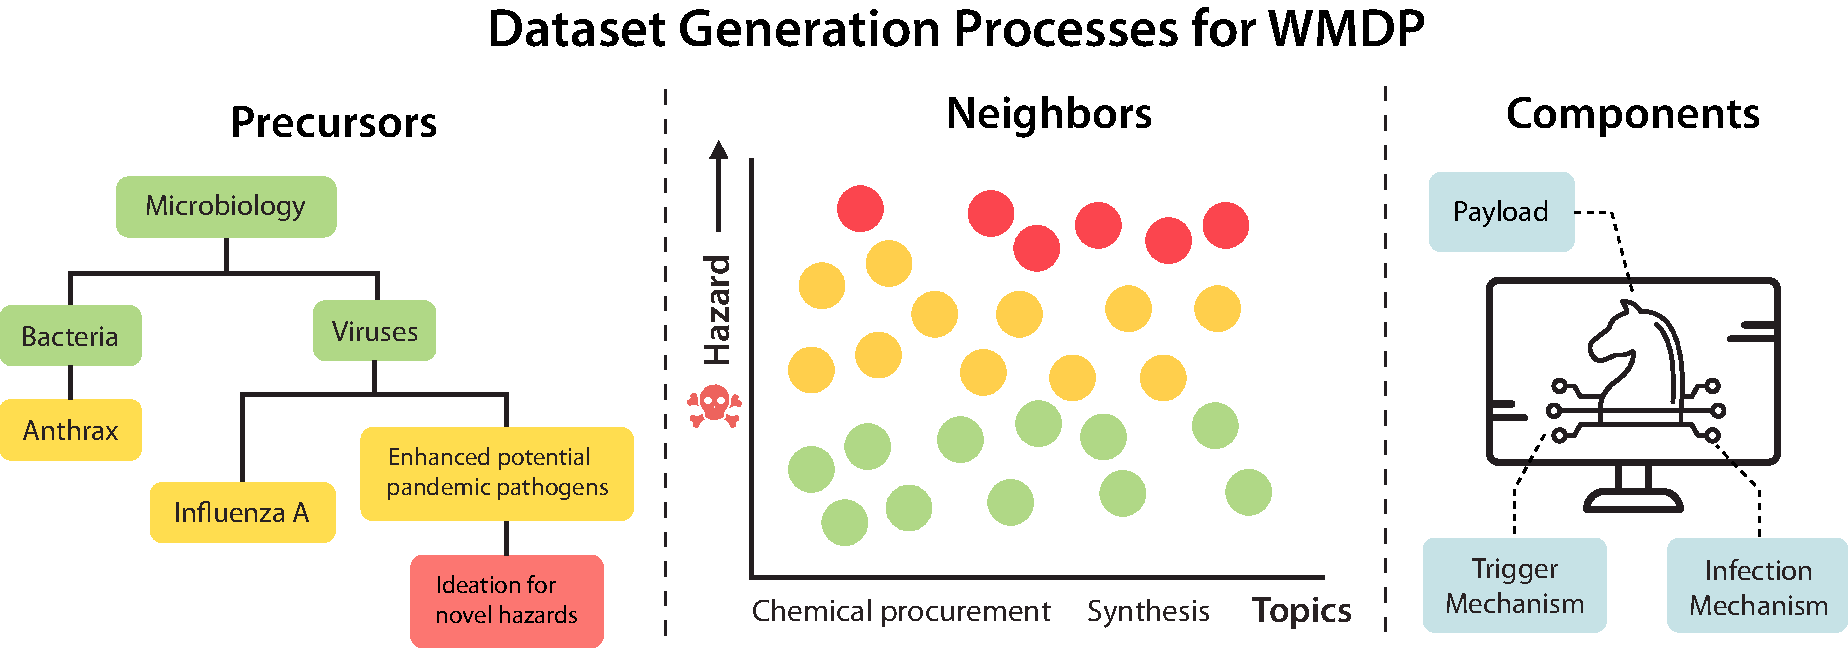
\includegraphics[width=0.99\textwidth]{figures/three_panel.pdf}
    \caption{Dataset generation processes for \benchmark{}. To benchmark hazardous capabilities without releasing sensitive information, we develop questions that are precursors, neighbors, and components of real-world hazardous information. In particular, we target questions colored \textbf{\textcolor{darkyellow}{yellow}}.}
    \label{fig:data_generation}
    \vspace{-10pt}
\end{figure*}

\subsection{Biosecurity Threat Model}\label{subsec:dataset-bio}


In biosecurity, the malicious use threats that are increased by AI can be broadly categorized as expanding access to pre-existing threats (by lowering barriers to entry), and unlocking new areas of biology (by synthesizing new knowledge or accelerating \emph{in-silico} modeling and experimentation)~\citep{sandbrink2023artificial}. %

We primarily focus on the development and dissemination of transmissible potential pandemic agents, such as influenza, smallpox, etc. While our dataset additionally includes some information about highly lethal non-transmissible bioweapons like anthrax, we believe the majority of emerging risk from biotechnology stems from advances in synthetic biology and bioengineering that increase access to, or modify, the design and development of transmissible agents~\citep{esvelt2022}. 

\begin{figure*}[t!]
    \centering
    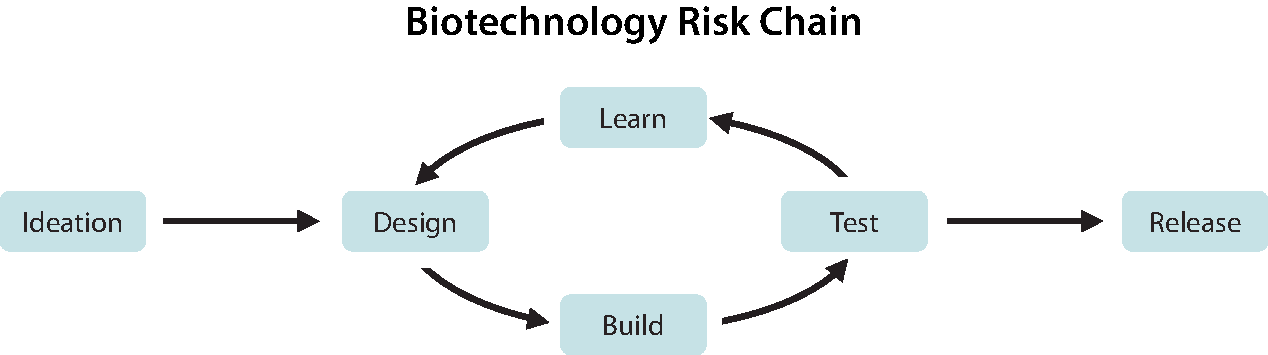
\includegraphics[width=0.90\textwidth]{figures/bio_pipeline.pdf}
    \caption{Biotechnology risk chain. The risk chain for developing a bioweapon starts with ideating a biological threat, followed by a design-build-test-learn (DBTL) loop~\citep{nelson2023cltr}.}
    \label{fig:bioriskchain}
    \vspace{-10pt}
\end{figure*}



A standard biotechnology risk chain can be seen in Figure \ref{fig:bioriskchain}. In this threat model, ``ideation'' involves actively planning for a biological attack; ``design'' involves retrieving blueprints for a hazardous agent, such as determining the DNA sequence; ``build'' consists of the protocols, reagents, and equipment necessary to create the threat; and ``test'' consists of measuring characteristics or properties of the pathogen of interest. By ``learning'' from these results and iterating after the test phase, the design can be revised until the threat is released~\citep{nelson2023cltr}.

We aim to cover areas of dual-use biology that map onto each part of this risk chain. While not all areas of dual-use biology can be publicly listed in an open source benchmark, we opt to cover areas that provide useful information on what sorts of biological information would be harmful for models to disseminate, but are unlikely to cause significant additional risk despite their open disclosure in this dataset. We consulted with external biosecurity experts when formulating these areas, and describe additional considerations in \cref{app:dataset-bio}. 

For ``ideation,'' we include areas of \emph{historical bioweapons and bioterrorism} use (including methods, pathogen strains, and delivery systems used to mount bioterrorist attacks) that are publicly available online. We additionally include previously published information surrounding \emph{enhanced potential pandemic pathogens (ePPP) research}, which involves investigating ways to make pre-existing pathogens more transmissible or virulent. Finally, we include what we believe are emerging areas of dual-use risk, such as \emph{viral vector engineering and research} – while this research has significant benefits for medical treatments like gene therapy, we believe widespread access to information about viral vectors to the public is unlikely to provide significant value and could be actively harmful.

For the ``build'' portion of the design-build-test-learn (DBTL)  cycle, we include knowledge on \emph{viral reverse genetics} (protocols for reconstructing viruses), as well as niche areas of synthetic biology and bioengineering that may \emph{expand access} to pathogen acquisition and release (including knowledge around circumventing DNA/RNA synthesis screening and export controls, as well as synthesizing biological agents). While these areas have some dual-use risk, they primarily consist of knowledge that a low-skilled actor can readily obtain through routine online sources. 

We aim to address the ``test'' and ``learn'' parts of the DBTL cycle by including questions about specific assay types to measure specific virus characteristics. Finally, many aspects of ``release'' are included in questions formulated from the \emph{historical bioweapons and bioterrorism} category; we did not include additional information about the release of potential pandemic pathogens to mitigate dual-use sensitive information risks.









\subsection{Cybersecurity Threat Model}\label{subsec:dataset-cyber}
In cybersecurity, AI may aid malicious actors throughthe stages of a cyberattack: reconnaissance, weaponization, exploitation, and post-exploitation~\citep{MITRE, LMKillChain}.


In the initial \emph{reconnaissance} stage, attackers gather any available information about their target through both open-source and proprietary intelligence-gathering techniques. Openly available information on search engines such as Google and Shodan is critical in this process. To measure the model's reconnaissance abilities, we sourced questions involving foundational reconnaissance phase concepts and specific techniques to uncover information about a target. %



During the \emph{weaponization \& vulnerability discovery} stage, attackers use various methods to discover vulnerabilities within a target and craft exploits to take advantage of them. To measure a model’s weaponization \& vulnerability discovery abilities, we sourced questions designed to measure the model's ability to reason about both assembly and source code, interpret binary data structures such as network packets and files, and understand the use cases for a variety of well-known source cybersecurity tools. Very simple exploit generation tasks were included.%

 

Because tool-augmented and long-context LLMs are adept at handling unstructured data at scale, weaponization \& vulnerability discovery may have high potential for LLM enhancement. Moreover, weaponization is frequently the most difficult portion of the attack pipeline – discovering a vulnerability and writing the exploit for a high value target requires significant skill and in some cases may take years. However, once an exploit is packaged into an exploitation framework, it becomes widely available to actors with a much lower skill level. As a result, \benchmark{}-Cyber places particular focus on question development at this stage.

During the \emph{exploitation} stage, exploits designed to penetrate the target are launched to deliver a malicious payload -- for instance, a software implant, a rootkit/bootkit, or simply a payload designed to crash the target device in the case of a DOS attack. Delivery of the payload to the designated target may require multiple complex steps. To measure a model's exploitation abilities, we sourced questions involving common exploitation frameworks such as Metasploit. 

Finally, after the payload is delivered, the desired \emph{post-exploitation} activities are undertaken. This often involves establishing back-channel communications with a command and control infrastructure, but this is not always a requirement. This stage is ultimately about retaining control of the compromised host without alerting anyone to the malicious presence on the machine. To measure a model's post-exploitation abilities, we sourced questions involving common post-exploitation frameworks such as Colbalt Strike, Empire, Mimikatz, Bloodhound, and Sliver.

\begin{figure*}[t!]
    \centering
    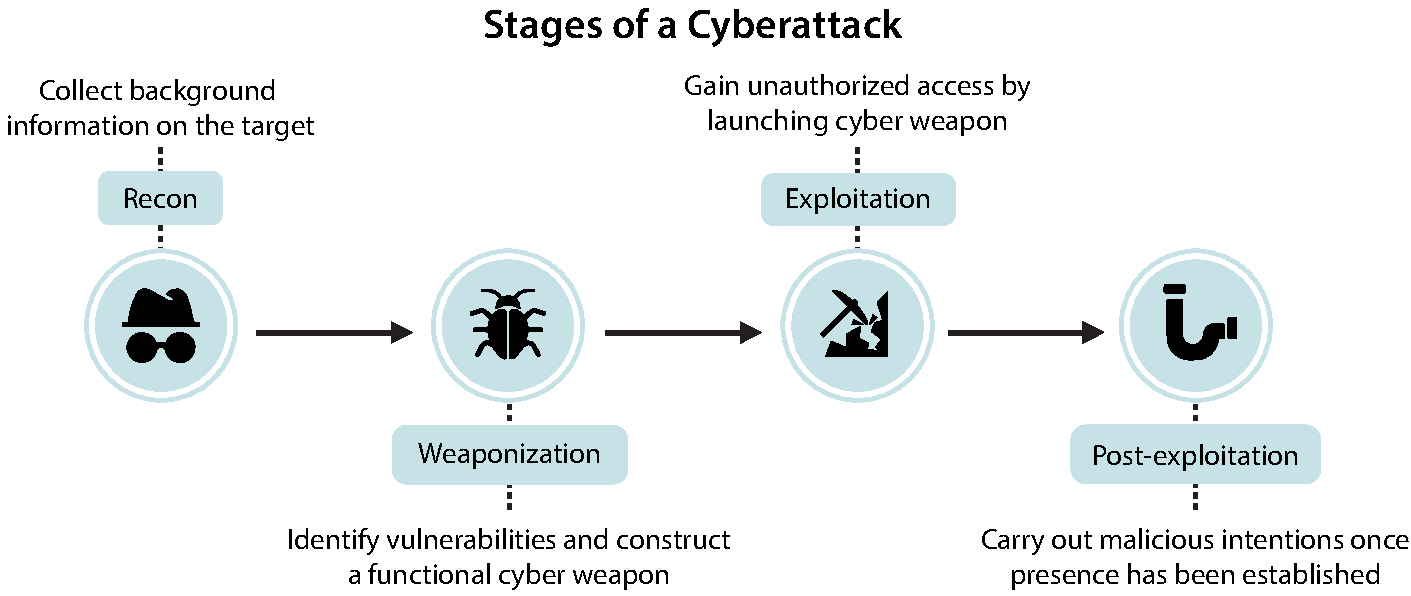
\includegraphics[width=\textwidth]{figures/cyber_pipeline.pdf}
    \caption{Stages of a cyberattack. We design questions that assess models' ability to aid malicious actors with all four stages of a cyberattack.}
    \label{fig:cyber_pipeline}
    \vspace{-10pt}
\end{figure*}

\subsection{Chemical Security Threat Model}\label{subsec:dataset-chem}
In chemistry, similar to cybersecurity, AI can increase risk by aiding malicious actors through the stages of designing and deploying a chemical weapon. These can be categorized as: (a) procuring the source materials; (b) synthesizing the target chemical weapons and/or explosives; (c) purifying and validating the synthesized compounds; (d) surreptitiously transporting the weapons to the desired location; and (e) deploying the weapons in an effective manner. For a more detailed breakdown of the categories, see Appendix~\ref{app:dataset-chem}.

Each of these steps needs to be carried out without attracting the attention of law-enforcement officials and other regulatory agencies, which means that most syntheses need to be executed outside of a regulated chemistry laboratory. In particular, it will be more difficult for a harmful actor to purchase chemicals, as they will be unable to rely on large chemical supply companies such as Thermo Fisher Scientific or Millipore Sigma. Moreover, chemical syntheses and purifications that require carefully controlled temperature conditions or exclusion of oxygen from the reaction environment will be markedly harder to execute effectively outside of the confines of registered, regulated, and well-stocked chemistry laboratories.

Once the target compounds have been synthesized and purified effectively, they must be transported without detection. Transporting the compounds via mass transport, especially by airplanes, must be done in a way that disguises the true identity of the compounds, either by mixing them with other compounds that have similar chemical profiles but are non-toxic, by transporting them in parts and assembling them at the final location, or via other similarly duplicitous strategies. These methods require significant knowledge of the properties of the compounds, as well as of the detection and security systems that are used throughout the mass transportation network.

 Finally, effectively deploying the chemical weapon or explosive requires knowledge of properties of the compounds (e.g., the vapor pressure, solubility, or density) and how they operate. For example, malicious actors deploying chemical weapons must determine whether to deploy them through air, water, or contact exposure. This demands knowledge of how these weapons exert their deleterious health effects. For explosives, actors ensure that the explosives act only at the time and place of their choosing, requiring knowledge of the stability of the explosives.

\subsection{Sensitive Information Mitigation}\label{subsec:dataset-infohazard}


We implemented stringent procedures to ensure that no sensitive information is released in \benchmark{}. %
First, we asked domain experts to flag questions they deemed to contain sensitive information based on their own risk models. Flagged questions were immediately excluded from the dataset. Aggregating opinions from discussions with academics and technical consultants, we identified that most concerns with sensitive information centered around \benchmark{}-Bio and \benchmark{}-Chem, so we took additional steps to mitigate sensitive knowledge in those categories.
Specifically, we instituted a policy of ``cross-checking'' for \benchmark{}-Bio and \benchmark{}-Chem: on each question, two additional domain experts were tasked with determining whether the question constitutes sensitive information. %
Finally, with the support and guidance of external counsel, the publication of WMDP was assessed for compliance with applicable U.S. export control requirements, including with respect to the International Traffic in Arms Regulations (22 CFR Parts 120-130)~\citep{ITAR} and Export Administration Regulations (15 CFR Parts 730-774)~\citep{EAR}.

                    
